
\documentclass{article}



\usepackage{graphicx,comment,framed}
\usepackage{roundbox}
\usepackage{fancybox}
\usepackage{tikz}
\usepackage{color}
\usepackage[hidelinks]{hyperref}
\usepackage{framed}
\usepackage{amsthm,amssymb,amsmath}
%\usepackage[colorlinks,linkcolor=blue,citecolor=blue]{hyperref}
\definecolor{shadecolor}{cmyk}{0,0,0,0}
\usepackage{listings}
\usepackage{xepersian}
\usepackage[noend]{algpseudocode}


%--------------------- page settings ----------------------

\settextfont[Scale=1.1]{XB Niloofar}
\setdigitfont[Scale=1.1]{XB Niloofar}
\defpersianfont\sayeh[Scale=1.1]{XB Niloofar}
\addtolength{\textheight}{3.2cm}
\addtolength{\topmargin}{-22mm}
\addtolength{\textwidth}{3cm}
\addtolength{\oddsidemargin}{-1.5cm}


%------------------------ Environments ------------------------------------

\newtheorem{قضیه}{قضیه}
\newtheorem{لم}{لم}
\newtheorem{مشاهده}{مشاهده}
\newtheorem{تعریف}{تعریف}


%-------------------------- Notations ------------------------------------
\renewcommand{\labelitemi}{$\bullet$}
\newcommand{\IR}{\ensuremath{\mathbb{R}}} 
\newcommand{\IZ}{\ensuremath{\mathbb{Z}}} 
\newcommand{\IN}{\ensuremath{\mathbb{N}}} 
\newcommand{\IS}{\ensuremath{\mathbb{S}}} 
\newcommand{\IC}{\ensuremath{\mathbb{C}}} 
\newcommand{\IB}{\ensuremath{\mathbb{B}}} 

\newcommand{\bR}{\mathbb{R}}
\newcommand{\cB}{\mathcal{B}}
\newcommand{\cO}{\mathcal{O}}
\newcommand{\cG}{\mathcal{G}}
\newcommand{\rM}{\mathrm{M}}
\newcommand{\rC}{\mathrm{C}}
\newcommand{\rV}{\mathrm{V}}

\newcommand{\lee}{\leqslant}
\newcommand{\gee}{\geqslant}
\newcommand{\ceil}[1]{{\left\lceil{#1}\right\rceil}}
\newcommand{\floor}[1]{{\left\lfloor{#1}\right\rfloor}}
\newcommand{\prob}[1]{{\mbox{\tt Pr}[#1]}}
\newcommand{\set}[1]{{\{ #1 \}}}
\newcommand{\seq}[1]{{\left< #1 \right>}}
\newcommand{\provided}{\,|\,}
\newcommand{\poly}{\mbox{\rm poly}}
\newcommand{\polylog}{\mbox{\rm \scriptsize polylog}\,}
\newcommand{\comb}[2] {\left(\!\!\begin{array}{c}{#1}\\{#2}\end{array}\!\!\right)}




\newcounter{probcnt}
\newcommand{\مسئله}[1]{\stepcounter{probcnt}{
 	\bf \arabic{probcnt}$\mbox{\bf{.}}$ \ #1}}

\newcommand{\fqed}[1]{\leavevmode\unskip\nobreak\quad\hspace*{\fill}{\ensuremath{#1}}}

\newenvironment{اثبات}
	{\begin{trivlist}\item[\hskip\labelsep{\em اثبات.}]}
	{\fqed{\square}\end{trivlist}}

\newenvironment{حل}
	{\begin{trivlist}\item[\hskip\labelsep{\bf حل.}]}
	{\fqed{\blacktriangleright}\end{trivlist}}

\ifdefined\hidesols
	\newsavebox{\trashcan} % uncomment the following line to hide solutions
	\renewenvironment{حل}{\begin{latin}\begin{lrbox}{\trashcan}}{\end{lrbox}\end{latin}}
\fi


%------------------------- Header -----------------------------

%------------------------- Header -----------------------------

\newcommand{\سربرگ}[3]{
	\parindent=0em
	
	
	\begin{shaded}
		
		\rightline{ 
			\makebox[8em][c]{
				
\includegraphics[height=3cm]{aut.png}
		}} \ \
	\\[-3em] 
	\centerline{ مدرس :دکتر امیر مزلقانی } 
	\\[-6.5em]
	\centerline{\large \bf جبرخطی کاربردی }
	\\[0.05em]
	\centerline {\bf نیمسال دوم 98-97}	
	\\[-6.4em]
		\leftline{ 
		\makebox[8em][c]{
			
\includegraphics[height=3.2cm]{ceit.jpg}
	}}
	
	
		

		\hrule height .12em
		
		\normalsize
		\vspace{1mm} #1
		\hfill \small  #3
		\vspace{1mm} 
		\hrule height .1em
		
		\vspace{-0.5em} 
		\hfill {\sayeh\large #2} \hfill
	\end{shaded}
	
{\bf توجه !!!}	
\begin{itemize}
	\item 
	سوالات زیر مربوط به فصل اول درس جبر خطی کاربردی با موضوع ((معادلات خطی در جبر خطی )) می باشد که شامل 5 سوال تئوری و 2 سوال عملی است
	\item 
	سوالات را به دقت و مطالعه و به صورت خوانا و مرتب بنویسید
	\item 
	مهلت ارسال این تمرین ساعت 
	\color{red}{23:55 روز شنبه 97/12/18}
	می باشد. 
\end{itemize}
}





\begin{document}
\سربرگ{پاسخ تمرین سری 3}{}{}

\مسئله{}
در هر مورد مشخص کنید آیا زیر مجموعه ی داده شده یک زیر فضا از فضای برداری مشخص شده می باشد یا خیر.
\begin{enumerate}
	\item 
	تمامی زوج مرتب هایی مثل
	$(x,y)$
	از 
	$\mathbb{R}^2$
	با اعمال جمع برداری و ضرب اسکالر زیر:
	
	$$(x,y)+(x',y')=(x+x',0),c(x,y)=(cx,0)$$
	\item
	$\{(a,b,a+b)|a,b\in \mathbb{R}  \}$
	در فضای برداری 
	$\mathbb{R}^3$.
	\item
	$\{A\in M_n(\mathbb{R})|\det(A)=0\}$
	در
	$M_n(\mathbb{R})$.
	(منظور از 
	$M_n(\mathbb{R})$
	مجموعه تمام ماتریس های 
	$n\times n$
	با درایه هایی از مجموعه اعداد حقیقی است.)
	
	\item 
	$\{p(x)|p(x)=p(-x),p(x)\in\mathbb{P} [x]  \}$
	در فضای برداری 
	$\mathbb{P}[x]$
	(تمامی چند جمله های حداکثر از درجه 
	$n$
	با ضرایب حقیقی را با نماد  
	$\mathbb{P}_n[x]$
	نشان می دهیم و همچنین مجموعه تمام چند جمله ها با ضرایب حقیقی را با  
	$\mathbb{P}[x]$
	نشان می دهیم) 
	\item 
	$\{p(x)|p(x)=ax^2,a\in\mathbb{R}\}$
	در فضای برداری 
	$\mathbb{P}_3[x]$.
	
\end{enumerate}

\مسئله{}
اگر 
$V,W$
فضا ها برداری باشند،
$V\times W$
تمام زوج مرتب هایی به شکل 
$(v,w)$
است که 
$v\in V,w\in W$
و تعریف می کنیم:
$$(v_1,w_1)+(v_2,w_2)=(v_1+v_2,w_1+w_2)$$
و 
$$k(v,w)=(kv,kw),\qquad k\in \mathbb{R}$$
\begin{enumerate}
\item 	
	نشان دهید 
	$V\times W$
	یک فضای برداری است.
	\item  
	نشان دهید اگر بعد 
	$V$
	و
	$W$
	متناهی باشد آنگاه بعد 
	$V\times W$
	نیز متناهی است.
	\item 
	بعد 
	$V\times W$
	را در صورتی که 
	$dimV=m,dimW=n$
	بیابید.
	\item 
	توضیح دهید چرا 
	$\mathbb{R}\times \mathbb{R}^2$
	با 
	$\mathbb{R}^3$
	یکسان است.
	\item 
	پایه ای برای 
	$\mathbb{R}^2\times M_2(\mathbb{R})$
	بیابید.
	\item 
	بعد 
	$M_2(\mathbb{R})\times M_2(\mathbb{R})$
	را بیابید.
\end{enumerate}
\begin{حل}
	\begin{figure}[h]
		\centering
		
		‎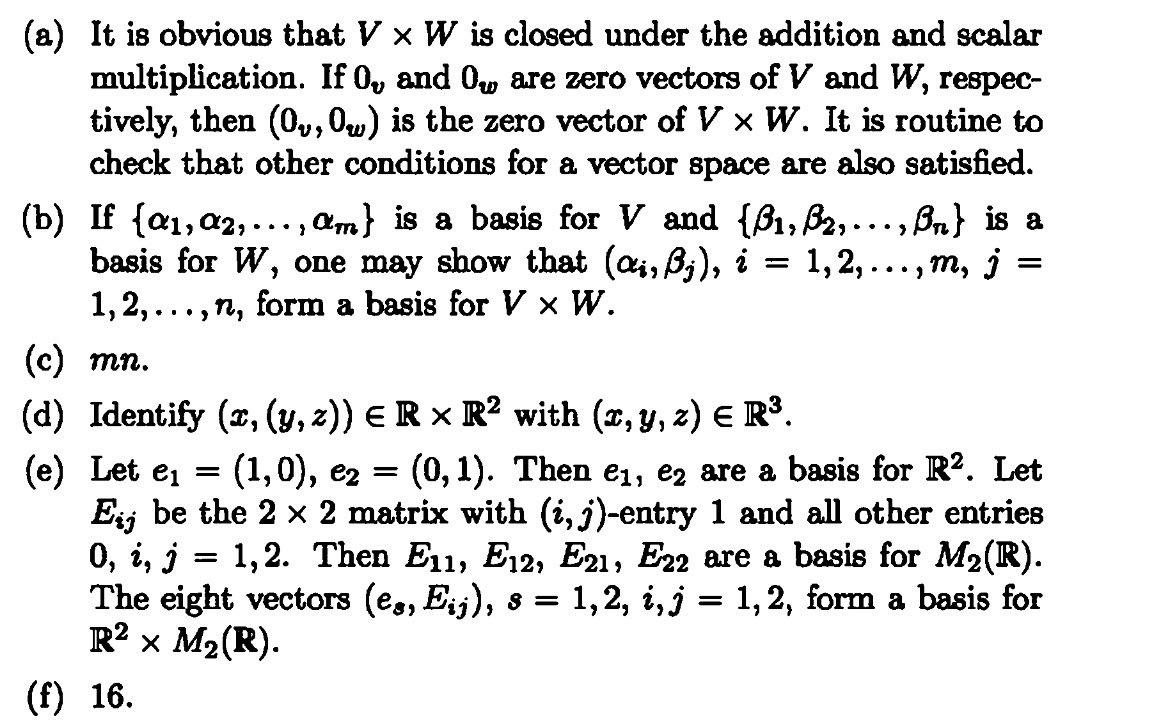
\includegraphics[scale=0.5]{abc}‎
	\end{figure}    
	\end{حل}
\مسئله{}
فرض کنید 
$W_1,W_2$
زیر فضا های فضای برداری 
$V$
باشند، تعریف می کنیم :
$$W_1+W_2=\{w_1+w_2|w_1\in W_1,w_2\in W_2\}$$.

\begin{enumerate}\item 
	نشان دهید :
	$$W_1+W_2+\cdots+W_n=span(\bigcup_{i=1}^{n}W_i)$$
	\begin{حل}
		$$v\in W_1+W_2+\cdots+W_n\longleftrightarrow \exists \ \ w_1,w_2,\cdots,w_n \quad w_1\in  W_1,w_2\in  W_2,\cdots w_n\in W_n \quad v=w_1+w_2+\cdots+w_n$$
		$$\longleftrightarrow w_1,w_2,\cdots,w_n\in\bigcup_{i=1}^{n}W_i\longrightarrow w_1+w_2+\cdots+w_n\in span(\bigcup_{i=1}^{n}W_i)\longleftrightarrow v\in span(\bigcup_{i=1}^{n}W_i) $$	
	\end{حل}
	\item 
	نشان دهید 
	$W_1\cap W_2,W_1+W_2$
	زیر فضای 
	$V$
	هستند و همچنین نشان دهید:
	$$W_1\cap W_2 \subseteq W_1\cup W_2\subseteq W_1+W_2$$.
	\begin{حل}
		می دانیم 
		$0\in W_1,0\in W_2$
		پس 0 عضو 
		$W_1+W_2$
		هست از سوی دیگر 
		\\
		اگر 
		$v_1\in W_1+W_2,v_2\in W_1+W_2$
		باشد،آنگاه طبق تعریف داریم :
		$$\exists w_1\in W_1,w_2\in W_2 \ \ v_1=w_1+w_2\quad,\quad \exists w'_1\in W_1,w'_2\in W_2 \ \ v_2=w'_1+w'_2$$
		در نتجه:
		$$v_1+v_2=w_1+w_2+w'_1+w'_2=\underbrace{w_1+w'_1}_{\in W_1}+\underbrace{w_2+w'_2}_{\in W_2}\longrightarrow v_1+v_2\in W_1+W_2$$
		همچنین باید ثابت کنیم اگر 
		$v\in W_1+W_2$
		باشد آنگاه 
		$kv$
		هم چنین است که 
		$k$
		یک اسکالر است.
		$$\exists w_1\in W_1,w_2\in W_2 \ \ v=w_1+w_2\longrightarrow kv=\underbrace{kw_1}_{\in W_1}+\underbrace{kw_2}_{\in W_2}\longrightarrow kv\in W_1+W_2$$
		پس 
		$W_1+W_2$
		یک زیر فضای 
		$V$
		است.
		
		حال باید ثابت کنیم 
		$W_1\cap W_2 $
		زیر فضای 
		$V$
		است. می دانیم صفر عضو هر دو زیر فضا است پس صفر در اشتراک آن ها نیز وجود دارد،حال باید ثابت می کنیم که :
		$$v_1\in W_1\cap W_2, v_2\in W_1\cap W_2\longrightarrow v_1\in W_1\wedge v_1\in W_2, v_2\in W_1,v_2\in W_2$$$$\longrightarrow v_1+v_2\in W_1\wedge v_1+v_2\in W_2\longrightarrow v_1+v_2\in W_1\cap W_2 $$
		به همین شکل ثابت می شود ضرب یک اسکالر در اعصای 
		$W_1\cap W_2$
		عضو 
		$W_1\cap W_2$
		است پس زیر فضا بودن اشتراک دو زیر فضا نیز ثابت می شود.
		
		اکنون باید ثابت کنیم رابطه بالا برقرار است بدیهی است که اشتراک دو زیر فضا زیر مجموعه اجتماع آن است (این رابطه برای هر دو مجموعه ای فارغ از زیر فضا بودن یا نبودن صادق است) کافی است ثابت کنیم: 
		$$W_1\cup W_2\subseteq W_1+W_2$$
		برای اثبات این موضوع از رابطه قسمت 1 استفاده می کنیم، طبق قسمت 1 می دانیم: 
		$$W_1+W_2=span(W_1\cup W_2)$$
		واضح است که اگر مجموعه ای به شکل 
		$A$
		داشته باشیم آنگاه:
		$$A\subseteq span(A)$$
		زیرا :
		$$span(A)=\lambda_1a_1+\lambda_2 a_2+\cdots+\lambda_n a_n\qquad \lambda_i\in \mathbb{R},a_i\in A$$
		و فرض کنید در هر مرحله 
		$(\lambda_i=1)$
		و 
		$(\lambda_j=0 , j\neq i)$
		در این صورت 
		$A\subseteq span(A)$.
	\end{حل}
	\item 
	نشان دهید :
	$$dim(W_1+W_2)=dim(W_1)+dim(W_2)-dim(W_1\cap W_2)$$.
	\begin{حل}
		فرض کنیم :
		$$diam W_1=n,dim W_2=m,dim(W_1\cap W_2)=t$$
		همچنین فرض کنید:
		$\{u_1,u_2,\cdots,u_t\}$
		یک پایه برای 
		$W_1\cap W_2$
		باشد،پس می توان آنرا به یک پایه 
		\\
		$B_1=\{u_1,u_2,\cdots,u_t,v_1,v_2,\cdots,v_{n-t}\}$
		از 
		$W_1$
		و همچنین  
		$B_2=\{u_1,u_2,\cdots,u_t,w_1,w_2,\cdots,w_{m-t}\}$
		از 
		$W_2$
		توسعه داد.ثابت می کنیم:
		$$B=\{u_1,u_2,\cdots,u_t,v_1,v_2,\cdots,v_{n-t},w_1,w_2,\cdots,w_{m-t}\}$$
		یک پایه برای 
		$W_1+W_2$
		است.که رد این صورت حکم مسئله نیز ثابت می شود ،برای اثبات پایه بودن باید استقلال خطی و مولد بودن را ثابت می کنیم(مولد بودن یعنی ترکیب های خطی یک مجموعه تمامی اعضای آن مجموعه را تولید می کنند که در واقع بیانگر این است که اگر 
		$if\ \ A\subseteq B\to span(A)=B$
		در بحث ما می گوییم بردار هایی مولد یک فضا یا زیر فضا هستند که تمامی اعضای آن ها را بتوان با ترکیب خطی این  بردار ها تولید کرد.
		)
		\\
		{\bf  استقلال خطی :}
		$$\sum_{i=1}^{t}\alpha_iu_i+\sum_{i=1}^{n-t}\beta_i v_i+\sum_{i=1}^{m-t}\gamma_i w_i=0(\star)\longrightarrow \underbrace{\sum_{i=1}^{t}\alpha_iu_i+\sum_{i=1}^{n-t}\beta_i v_i}_{\in W_1}=\underbrace{\sum_{i=1}^{m-t}-\gamma_i w_i}_{\in W_2} $$
		$$\longrightarrow \sum_{i=1}^{m-t}-\gamma_i w_i\in W_1\cap W_2 $$
		پس وجود دارد 
		$\mu_1,\mu_2,\cdots,\mu_t$
		به طوری که:
		$$\sum_{i=1}^{m-t}-\gamma_i w_i=\sum_{i=1}^{t}\mu_iu_i$$
		$$\longrightarrow \sum_{i=1}^{m-t}\gamma_i w_i+\sum_{i=1}^{t}\mu_iu_i=0$$
		چون ترکیب خطی فوق صفر ،
		$\mu_i$
		ها ،
		$w_i$
		ها یک پایه برای 
		$w_2$
		و ذا مستقل خطی هستند 
		
		پس :
		$\forall i\ \ \gamma_i=0,\forall i\ \ \mu_i=0$
		با جایگذاری در 
		$\star$
		داریم :
		$$\sum_{i=1}^{t}u_i+\sum_{i=1}^{n-t}=0$$
		یعنی ترکیب خطی از اعضای پایه 
		$W_1$
		صفر شده است ،پس :
		$$\forall i \alpha_i=0,\forall i \beta_i=0$$
		پس 
		$B$
		مستقل خطی است.
		
		{\bf  مولد بودن:}
		باید ثابت کنیم هر 
		$w\in W_1+W_2$
		را می توان به صورت ترکیب خطی 
		$B$
		نوشت.
		
		می دانیم طبق تعریف :
		$$\exists w'_1\in W_1,w'_2\in W_2\quad w=w'_1+w'_2$$
		$$\longrightarrow w'_1=\alpha_1u_1+\alpha_2u_2+\cdots+\alpha_tu_t+\alpha_{t+1}v_1+\alpha_{t+2}v_2+\cdots+\alpha_{n}v_{n-t}$$
		$$\longrightarrow w'_2=\beta_1u_1+\beta_2u_2+\cdots+\beta_tu_t+\beta_{t+1}w_1+\beta_{t+2}w_2+\cdots+\beta_{m}w_{m-t}$$
		\begin{align*}\longrightarrow w=w'_1+w'_2=&(\alpha_1+\beta_1)u_1+(\alpha_2+\beta_2)u_2+\cdots+(\alpha_t+\beta_t)u_t+\\&\alpha_{t+1}v_1+\alpha_{t+2}v_2+\cdots+\alpha_{n}v_{n-t}+\beta_{t+1}w_1+\beta_{t+2}w_2+\cdots+\beta_{m}w_{m-t}
		\end{align*}
		پس توانستیم 
		$w$
		را برحسب 
		$B$
		بنویسیم و در نتیجه 
		$B$
		مولد و مستقل خطی است و پایه است و حکم ثابت می شود.
	\end{حل}
	\item 
	نتیجه گیری قسمت 
	$2$
	را با استفاده از دو خط که از مبدا مختصات 
	$xy$
	می گذرند توجیه کنید.
	\begin{حل}
		فرض کنید دو خط متقاطع داریم که در یک نقطه مشترکند،خط اول را با 
		$W_1$
		و خط دوم را با 
		$W_2$
		نشان می دهیم.
		آنگاه :
		$W_1\cap W_2$
		یک نقطه خواهد بود،و 
		$W_1\cup W_2$
		از خود این دو خط متقاطع تشکیل خواهد شد.در این صورت 
		$W_1+W_2$
		صفحه گذرنده از این دو خط خواهد بود.که رابطه 2 به وضوح با این فرضیات مشخص است.
	\end{حل}
	\item 
	چه زمانی 
	$W_1\cup W_2$
	زیر فضایی از 
	$V$
	است؟
	\begin{حل}
			\begin{figure}[h]
			\centering
			
			‎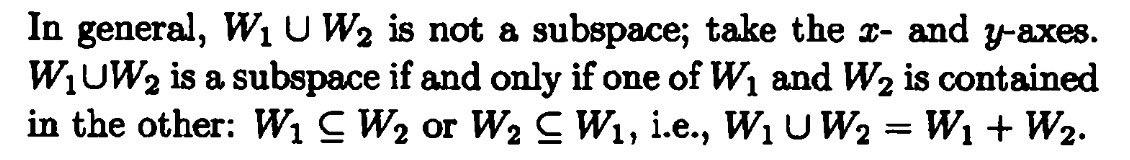
\includegraphics[scale=0.5]{abc1}‎
		\end{figure}    
		\end{حل}
	\item 
	اگر 
	$W_1+W_2$
	کوچکترین زیر فضایی از 
	$V$
	باشد که شامل 
	$W_1\cup W_2$
	است،و اگر 
	$S$
	زیر فضایی از 
	$V$
	باشد که شامل 
	$W_1\cup W_2$
	است آنگاه:
	$W_1+W_2\subseteq S$.
	\begin{حل}
			\begin{figure}[ht]
			\centering
			
			‎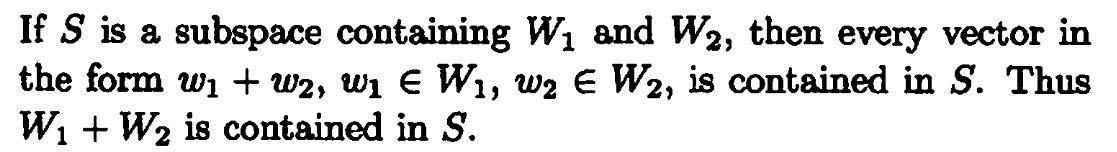
\includegraphics[scale=0.5]{abc2}‎
		\end{figure}    
		\end{حل}
	
\end{enumerate}
\مسئله{}
نشان دهید 
$\{u_1,u_2,\cdots,u_p\}$
در 
$V$
مستقل خطی هستند اگر و فقط اگر بردار های مختصات آن\\

$\{[u_1]_\mathcal{B},[u_2]_\mathcal{B},\cdots,[u_p]_\mathcal{B}\}$
در 
$\mathbb{R}^n$
مستقل خطی باشند.


\مسئله {} فرض کنید 
$S$
یک مجموعه متناهی در 
$V$
باشد به طوری که هر 
$x\in V$
نمایشی یکتا از ترکیب خطی اعضای 
$S$
داشته باشد،نشان دهید 
$S$
پایه 
$V$
است.
\begin{حل}
	قسمت 4.4 سوال 25.
	\end{حل}
\مسئله{}
با در نظر گرفتن 
$T:V\longrightarrow W$
فرض کنید 
$H$
زیر فضایی غیر صفر از 
$V$
باشد،و 
$T(H)$
مجموعه تمام بردار های تصویر شده 
$H$
باشد که زیر فضای 
$W$
است،ثابت کنید
$dim T(H)\leq dim H$.

\begin{حل}
	قسمت 5.4 سوال 31.
\end{حل}

\مسئله{}ماتریسی را 
(\lr {full rank})
گویند هرگاه رنک آن بزرگترین مقدار ممکن را داشته باشد،ثابت کنید ماتریس 
$m\times n$
که تعداد سطر های آن بیشتر از ستون هایش باشد 
\lr {full rank}
است اگر و فقط اگر ستون های آن مستقل خطی باشند. 
\begin{حل}
	قسمت 6.4 سوال 26.
\end{حل}
\مسئله {}اگر 
$A$
یک ماتریس 
$m\times n$
با رنک 
$r$
باشد آنگاه می گوییم 
$A=CR$
 یک 
(\lr{rank factorization})
ماتریس 
$A$
است هر گاه
$C$
یک ماتریس 
$m\times r$
با رنک
$r$
و 
$R$
یک ماتریس 
$r\times n$
با رنک 
$r$
باشد.چنین تقسیم بندی همیشه موجود است،با استفاده از این موضوع ثابت کنید برای هر دو ماتریس 
$m\times n$،
$A$
و
$B$،
نشان دهید:
$$rank(A+B)\leq rank A+rank B$$
\begin{حل}
	قسمت 
	\lr{supplementary exercises}
	سوال 16.
\end{حل}

\مسئله{}(سوال امتیازی)فرض کنید
$V$
 یک فضای برداری متناهی است و 
$V_1,V_2$
زیر فضا هایی از 
$V$
هستند.اگر 


$dim(V_1+V_2)=dim(V_1\cap V_2)+1$
آنگاه 
$V_1+V_2$
یا برابر 
$V_1$
است یا 
$V_2$
و متقابلا 
$V_1\cap V_2 $یا برابر 
$V_1$
است یا 
$V_2$.
هم ارز با جملات قبل اگر 
$V_1,V_2$
زیر مجموعه های هم نباشند،آنگاه:
$$dim(V_1+V_2)\geq dim(V_1\cap V_2)+2$$

\مسئله{}(سوال امتیازی)فرض کنید 
$U$
و
$V$
زیر فضا هایی از 
$R^n$
باشند به طوری که 
$$U=span\{\alpha_1,\alpha_2,\cdots,\alpha_p\}\qquad V=span\{\beta_1,\beta_2,\cdots,\beta_q\}$$
فرض کنید:
$$W=span\{\alpha_i+\beta_j\}\quad i=1,2,\cdots,p \quad j=1,2,\cdots,q$$
اگر 
$dimU=s, dim V=t$
نشان دهید:
$$dimW\leq min\{n,s+t\}$$


\مسئله {} در هر یک از قسمت های زیر ابتدا مختصات بردار داده شده
$(v)$ 
را در هریک از پایه ها بیابید سپس ماتریس انتقال از یک پایه
$(B)$
به پایه
$(C)$
دیگر را محاسبه کنید.
\begin{enumerate}
	\item 
	$$V=\mathbb{P}_3[x]\qquad v=p(x)=8+x+6x^2+9x^3$$
	$$B=\{−2+3x+4x^2-x^3, 3x+5x^2+2x^3, -5x^2-5x^3,
	4 + 4x + 4x^2\}$$
	$$C=\{1 - x^3, 1 + x, x + x^2, x^2 + x^3\}$$
	\item 
	$$V=M_2(\mathbb{R})\qquad v=\begin{bmatrix}
	-3&-2\\
	-1&2
	\end{bmatrix}
	$$
	$$B=\{
	\begin{bmatrix}
	1&0\\
	-1&-2
	\end{bmatrix}
	\begin{bmatrix}
	0&-1\\
	3&0
	\end{bmatrix}
	\begin{bmatrix}
	3&5\\
	0&0
	\end{bmatrix}
	\begin{bmatrix}
	-2&-4\\
	0&0
	\end{bmatrix}
	\}$$
	$$C=\{
	\begin{bmatrix}
	1&1\\
	1&1
	\end{bmatrix}
	\begin{bmatrix}
	1&1\\
	1&0
	\end{bmatrix}
	\begin{bmatrix}
	1&1\\
	0&0
	\end{bmatrix}
	\begin{bmatrix}
	1&0\\
	0&0
	\end{bmatrix}
	\}$$
	\item
	$$V=\mathbb{R}^3\qquad v=(1,7,7)$$
	$$B=\{(-7,4,4),(4,2,-1),(-7,5,0)\}$$
	$$C={(1,1,0),(0,1,1),(3,-1,-1)}$$
\end{enumerate}
 \begin{حل}
	برای حل این سوال قسمت دوم برای نمونه حل می شود حل دو قسمت دیگر نیز مشابه قسمت دوم می باشد که حل آن ها بر عهده خود شما دانشجویان گذاشته می شود.
	ابتدا مختصات 
	$v$
	را نسبت به پایه های 
	$B$
	و 
	$C$
	می یابیم.
	پس مختصات 
	$v$
	برحسب دو پایه برابراست با:
	$$[v]_B=(-1,-\frac{2}{3},-\frac{4}{3},-1)\qquad \qquad [v]_C=(2,-3,-1,-1)$$
	حال می خواهیم 
	$\underset{C\gets B}{P}$
	برای این کار باید ماتریس زیرا را تشکیل می دهیم:
	$$	\left(\begin{array}{cccc|cccc}
	1 & 1 & 1 & 1 & 1 & 0 & 3 & -2 \\ 
	1 & 1 & 1 & 0 & 0 & -1 & 5 & -4 \\
	1 & 1 & 0 & 0 & -1 & 3 & 0 & 0 \\
	1 & 0 & 0 & 0 & -2& 0 & 0 & 0$$ 
	
\end{array} \right)	$$

حال ماتریس سمت چپ به شکل کاهش یافته سطری پلکانی در می اوریم و اعمال سطری پلکانی مشابه را بر روی ماتریس سمت راست نیز اعمال می کنیم در نهایت ماتریس سمت راست همان 
$\underset{C\gets B}{P}$
خواهد بود.

\end{حل}
\end{document}


